\documentclass{article}
\usepackage[preprint]{ge2340_project}
\usepackage[utf8]{inputenc}
\usepackage[T1]{fontenc}
\usepackage{url}
\usepackage{booktabs}
\usepackage{longtable}
\usepackage{amsmath,amssymb}
\usepackage{graphicx}
\usepackage{microtype}
\usepackage{xcolor}
\usepackage{float}
\usepackage{hyperref}
\setcitestyle{numbers,square}
\hypersetup{colorlinks=true,linkcolor=blue,citecolor=blue,urlcolor=blue,
  pdftitle={Phase 2: Course Registration Helper for Balanced Workloads},pdfauthor={}}
\urlstyle{same}
\title{Phase 2: AI Project Report\\
\large Course Registration Helper for Balanced Workloads}
\author{}

\begin{document}
\maketitle

\section{Introduction \& Problem Recap}
Study-path planning is an important progress in university life.However, for some students in city university unfamiliar with GE or elective courses ,such as its background requirements, workload. While seats are limited, students often have to make a rush decision for which course to register. And there is a more often appears that: originally there is no seats at the before the semester start. After the first week, some other students in certain dropped the course, which free up the seats. However, the students who failed to register any GE courses ,rush to register the courses with new free space. But they may get into a course which difficult to them at week 2, where the add-drop period has been ended, make the decision become no no-regret.
Our helper uses an LLM and course scoring to suggest suitable, workload-aware schedules from students' interests, year and required courses. The prototype covers selected courses in one semester; it supports course selection rather than automatic registration or guaranteed seats.

Our design combines a fine-tuned language model with mathematical optimisation. The model interprets course information and proposes structured recommendations; source checks and an optimiser turn them into a constrained plan. This lets us personalise recommendations while respecting programme eligibility and academic dependencies.



\section{Data Collection \& Methodology}
\textbf{A programme-specific knowledge base.} Due to the time limitation and workload, we trained the data of BSc in Computing Mathematics (CM) and BSc in Computer science (CS) to the model.We assembled the student handbook, CM degree path and course list, CS major requirements and suggested plan, GE information, and saved Semester A/B timetable pages\citep{cityu-programmes}. We preserve source cohorts and academic years: the CM path concerns the 2025 intake, its designated course list is historical, and CS requirements and its suggested plan cover different academic-year contexts. These distinctions remain visible when rules need confirmation.

\begin{table}[H]
\centering\small
\caption{Coverage of our programme and timetable collection.}
\begin{tabular}{p{3.85in}r}
\toprule
Knowledge-base component & Coverage\\
\midrule
Distinct timetable files after duplicate removal & 93\\
Course--term--programme records & 86\\
Sections matching the encoded major restrictions & 128\\
CM / CS document-listed course codes & 85 / 73\\
GE codes in the original import & 64\\
Files excluded because meeting times were unrecognised & 7\\
\bottomrule
\end{tabular}
\label{tab:data}
\end{table}

\textbf{Turning documents into usable rules.} We extracted meeting days/times, prerequisites, exclusions and restrictions, removed duplicates and retained sources. ``ONLY FOR CM'' is an explicit major restriction. Candidates must appear in the student's designated programme document or the verified GE collection, then satisfy further eligibility checks. Entries with missing times are excluded from verified timetable planning. 

\newpage
\textbf{Training and evaluation design.} Our initial programme dataset contains 485 training, 24 validation and 30 test examples combining curriculum/timetable extraction with synthetic stream-policy answers. Its before/after comparison uses 15 preselected queries across membership, sections, course rules, source extraction and stream reasoning. The CM finance-background update uses 244 training and 32 validation examples, plus 20 held-out profile/candidate combinations. Both comparisons use the same base-loading protocol for each pair. Shared source facts and synthetic policies mean these are familiar-evidence tests, rather than unseen-cohort evaluations.

We complement this comparison with controlled penalty experiments, dependency interventions with fictional student profiles. Fictional transcripts let us vary academic histories without using real student records. Workload and preparation scores are transparent, editable estimates,with human feedback on the parameters. 

After the round of the training, we will give human feedback on the generated example to fine-tune the model further more.
\textbf{Prompts used in training.} Our saved training rows contain three message roles: a system instruction defining the task and output rules, a user message supplying the programme, passed courses, source facts and requested task, and an assistant message containing the target JSON. Instructions include ``Return JSON only,'' preserve source times, distinguish documents from instructions, count distinct stream slots, and never infer passes from year of study. The CM background prompt also states the EF/CS planning waiver and the treatment of failed/in-progress finance records. We train on assistant-answer tokens using supervised cross-entropy; this is more than providing a prompt at inference time.

\section{Implementation Details}
\textbf{From student profile to explained recommendation.} Our pipeline combines course evidence, the student's passed courses and their preferences. The language model returns structured proposals, which we check against exact local rules. The planner then evaluates eligible options and explains the selected route, reward contributions and unresolved requirements (Figure~\ref{fig:workflow}). A rejected model answer can be replaced by source lookup or exact policy calculation, with that intervention recorded separately.

\begin{figure}[H]
\centering
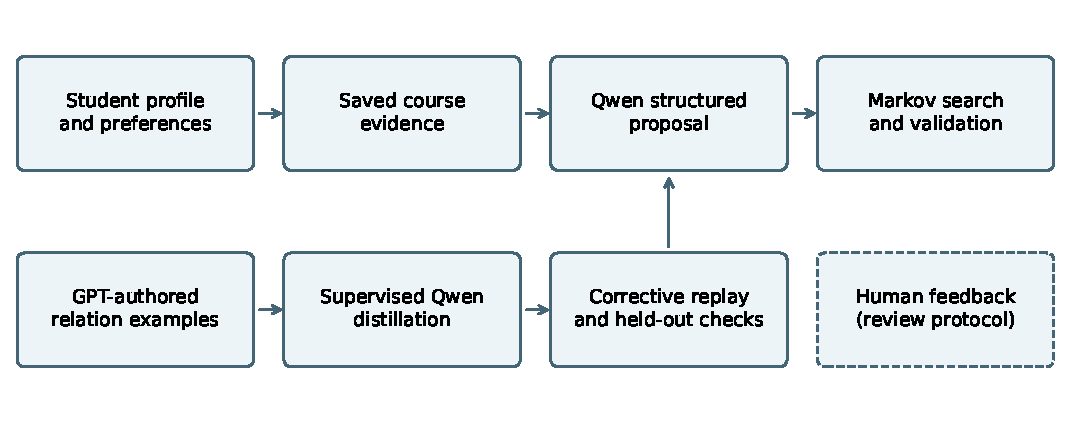
\includegraphics[width=\linewidth]{figures/workflow_training07.pdf}
\caption{Logged GPT-authored relation teaching, Qwen distillation and corrective replay feed source-based validation. Human feedback remains a separate review protocol.}
\label{fig:workflow}
\end{figure}

\begin{samepage}
\textbf{GPT teaching course relations.} The GPT assistant authored 26 directed preparation hypotheses using saved course aims, existing syllabus evidence and official catalogue descriptions. These are editable utility assumptions, rather than statistical correlations or measured workload reductions. Examples include MA2510 $\rightarrow$ MA3518 ($+0.30$), MA2503 $\rightarrow$ CS4487 ($+0.25$), MA3515 $\rightarrow$ EF3320 ($+0.25$), and finance GE $\rightarrow$ EF3320 ($+0.10$). The reward uses the strongest direct passed-source edge per target, capped at 0.35; it does not sum overlapping benefits, recurse through unstudied courses or award same-semester transfer. We distinguish this GPT-authored teacher from the separate GPT-6.1 Sol timetable comparator.

We distilled the policy into a separate Qwen relation checkpoint with 149 training and 20 validation examples over two epochs. Source-conditioned held-out checks improved from 17/20 to 20/20. A fresh three-source probe incorrectly summed three 0.25 benefits to 0.75; validation kept the correct 0.25. An 82-example corrective pass taught the maximum rule across passed-course combinations, fixed that familiar probe and retained 20/20 on the unchanged held-out set. The planner applies the checked policy, so neural arithmetic cannot inflate its reward.

\end{samepage}

\textbf{Human feedback after a full training round.} After one complete model-to-model teaching round and evaluation, a reviewer checks generated relations, rewards and schedules. Incorrect examples receive corrected targets and explanations; correct source examples are replayed to reduce forgetting. We then retrain Qwen and retain a checkpoint only if held-out checks support it. The repository demonstrates supervised training and corrective replay and now includes logged GPT-authored relation distillation and corrective trials. A formal human-annotation evaluation remains a protocol for the next review cycle.

\textbf{Efficient model adaptation.} We fine-tuned Qwen3-8B\citep{qwen} using rank-8 QLoRA\citep{qlora}, with a frozen four-bit base and BF16 computation. This adapts approximately 21.8 million parameters on a single RTX 5090. The finance-background fine-tune completed two epochs in approximately 5.5 minutes, with 7.37 GiB peak allocated GPU memory. Validation loss decreased from 0.13366 to 0.00135. We retained the first epoch because its validation result was better than the second.

We use supervised cross-entropy to teach structured responses. The planner's academic-profit objective is a separate optimisation function: training teaches the model to express the relevant information, while the optimiser decides which feasible course combination best fits the student's preferences. This separation makes preference changes immediate without requiring retraining.

\textbf{Input control.} Our local interface accepts a transcript profile, a desired stream, a stream-priority weight and three penalty weights. It provides course lookup, stream proposals, dependency paths and semester planning. The current planner uses deterministic Markov subset search over section bundles, with STOP unavailable below five credit-bearing courses in Years 1--3. It reports optimality only for unpruned searches; bounded searches report feasible output or search exhaustion. The earlier MILP implementation remains a reference baseline\citep{scipy}. We retain experiment inputs, outputs and policy decisions so recommendations can be traced back to the evidence\citep{runs}.

\newpage
\textbf{Reward and penalty function.} The three non-negative penalty weights express student priorities. We maximise net academic utility over feasible course sets using the following Markov-state objective.
\textbf{Final formula for the Markov decision process}
Let $s$ describe the student's completed courses, covered GE areas, year, credit progress and selected stream. For a feasible course set $X$, we maximise
\begin{align}
U(X,s)={}&\sum_{c\in X}\bigl[g_c(s)+p_c(s)+h_c(s)+q_c(s)\nonumber\\
&\quad-\lambda_b\bigl(b_c(s)+e_c(s)\bigr)-\lambda_d d_c(s)-\lambda_w w_c(s)\bigr]
+R_{\mathrm{stream}}(X,s)-O(X,s). \label{eq:utility}
\end{align}
The positive terms reward base course value $g$, preparation $p$, graduation priorities $h$, prerequisite bridges $q$ and progress towards one selected stream $R_{\mathrm{stream}}$. The three non-negative weights $\lambda_b,\lambda_d,\lambda_w$ control penalties for background mismatch, difficulty and workload. Here $e_c(s)=1.5$ for EF courses without finance-study evidence and zero otherwise. Profit is expressed in academic-utility points. Minimising the planner's loss is equivalent to minimising $-U$.
\\\textbf{overload penalty} To restrict the maximum credit that taken in a semester, we introduce overload penalty function
\begin{equation}
O(X,s)=\begin{cases}
0.25[\max(0,C(X)-15)]^2,&\text{Years 1--3},\\
0.25[\max(0,C(X)-12)]^2,&\text{Year 4}.
\end{cases}
\end{equation}
where $C(X)$ is semester credits. In Years 1--3 the penalty is zero through 15 credits, then 0.25 at 16 credits and 2.25 at 18 credits. In Year 4 it is zero through 12 credits, then 2.25 at 15 and 9 at 18 credits. We use the same 0.25 coefficient for the newly added earlier-year term. Inspection found that the previous default disabled overload penalties in Years 1--3; we corrected both the semester optimiser and the four-year simulation. This is a planner-policy correction, not a claim that the saved neural weights were retrained on this new threshold. The 18-credit hard limit remains separate.

\textbf{Personalisation across a degree} We use the logged GPT-authored content relationships to update preparation rewards. For example, a student who studied GE2340 can reward higher reward on furture AI -related course. Meanwhile, for GE course, if a student has already
covered its GE area, another distributional GE in that area receives only 0.3 base profit, encouraging breadth. A selected stream earns 2 points per new distinct requirement slot and a one-time 6-point completion reward. 

We account for both immediate progress and the next step in a course chain. For example, a prerequisite bridge can receive extra reward because it opens access to a preferred stream. Stream slots and completion rewards are counted once, including when several alternatives are selected together. In four-year simulations, the student's state is updated after each semester, allowing later decisions to reflect earlier choices.


\textbf{Background-focused CM planning.} For CM students, our planner allows an assumed prerequisite waiver for the listed EF and CS courses. Missing those formal passes adds no extra penalty. We instead assess finance preparation: background mismatch is 0.45 without evidence, 0.15 for introductory study and 0.05 for advanced passed study. Passed finance GEs or an explicit study declaration can supply introductory evidence; failed/in-progress courses do not. This is an advisory assumption, not verified university waiver approval.

\textbf{Academic requirements remain binding.} Programme membership, exclusions, required courses, credit bounds, section restrictions and timetable conflicts still apply. Mathematics and non-CM prerequisites remain enforced. Defaults require 5--6 courses in Years 1--3, with at most 18 credits; the Year 4 minimum is waived. Distributional GE is capped at one per semester, excluding compulsory language/development courses. Our CM degree simulation targets at least 122 credits, four distributional GEs spanning all three areas and at least 20 elective mathematics credits outside core/capstone study. The source's 122-credit threshold also meets the requested 121-credit minimum.

Unknown component linkage or teaching weeks is flagged. Hypothetical timetable examples explicitly state their assumptions, and dependency layers describe academic order rather than guaranteed future semester offerings. These boundaries help students distinguish a useful planning route from confirmed registration availability.

\newpage
\section{Results \& Evaluation}

\textbf{Updated Qwen--GPT comparison of timetable outputs.} We repeated the comparison after updating the GPT-authored preparation rewards. Eight synthetic end-of-Year-2 profiles are given a Year-3 Semester-A workload task: six familiar profiles and two additional missing-mathematics controls. Both models receive the same completed courses, exact snapshot option IDs, additive rewards, stream definitions and constraints. Neither sees the other model's output or the Markov reference. The GPT comparator is a separate agent configured as GPT-6.1 Sol; its provider-specific runtime revision is not exposed. Qwen uses the deployed timetable checkpoint and the updated preparation rewards; the checked teacher graph supplies the numeric preparation inputs, while the relation checkpoint is evaluated separately on expressing that policy.

The comparison uses the captured Semester-A term 202609 as a controlled workload scenario. It does not move those offerings into Semester A 2027 or certify a real future timetable. Table~\ref{tab:retest-input07} gives the complete profile and raw course selections. Table~\ref{tab:retest-path07} records the models' later academic-path explanations. Meeting times are checked for clashes but are omitted from the report tables.

\textbf{Completed-course bases for Table~\ref{tab:retest-input07}.} Each row lists its full passed-course history by base plus additions and explicit removals; no pass is inferred from year. 

\textit{CM base:} CS1302, CS2360, CS2468, GE1401, GE1501, GE2401, MA1300, MA1301, MA2503, MA2507, MA2508, MA2509, MA2510, MA3511, MA3526.

\textit{CS base:} CS1302A, CS2115, CS2310, CS2312, CS2402, CS3103, CS3201, CS3334, CS3342, GE1401, GE1501, GE1601, MA1503, MA1508, MA2185.

{\small
\setlength{\tabcolsep}{4pt}
\renewcommand{\arraystretch}{1.12}
\begin{longtable}{p{2.45in}p{1.35in}p{1.35in}}
\caption{Completed Year 2 profiles and raw Year 3 Semester-A workload selections under the updated rewards.}\label{tab:retest-input07}\\
\toprule
Year 2 completed-course profile & Fine-tuned Qwen & GPT-6.1 Sol\\
\midrule
\endfirsthead
\multicolumn{3}{l}{\textit{Continued}}\\
\toprule
Year 2 completed-course profile & Fine-tuned Qwen & GPT-6.1 Sol\\
\midrule
\endhead
\midrule
\multicolumn{3}{r}{\textit{Continued on next page}}\\
\endfoot
\bottomrule
\endlastfoot
{\raggedright \textbf{CM1; CM.} Passed: CM base; plus GE2260. \textit{Preference:} Financial Mathematics.\par} & {\raggedright MA3512, MA3518, MA3521, MA4542, MA4545\par} & {\raggedright MA3512, MA3518, MA3521, MA3525, MA4542\par}\\
\addlinespace[4pt]
{\raggedright \textbf{CM2; CM.} Passed: CM base except MA3526; plus GE2260. \textit{Preference:} Financial Mathematics.\par} & {\raggedright MA3512, MA3518, MA3521, MA3525, EF3320$^{\dagger}$. \textit{Rejected by validation.}\par} & {\raggedright MA3512, MA3518, MA3521, MA3525, MA4545\par}\\
\addlinespace[4pt]
{\raggedright \textbf{CM3; CM.} Passed: CM base; plus GE2260. \textit{Preference:} Enriched Mathematics.\par} & {\raggedright MA3512, MA3518, MA3525, MA4542, MA4545\par} & {\raggedright MA3512, MA3518, MA3525, MA4542, MA4545\par}\\
\addlinespace[4pt]
{\raggedright \textbf{CS1; CS.} Passed: CS base; plus GE2340. \textit{Preference:} Artificial Intelligence.\par} & {\raggedright CS3356, CS3383, CS3402, CS3483, CS4486$^{\dagger}$. \textit{Rejected by validation.}\par} & {\raggedright No feasible five-course plan in supplied pool\par}\\
\addlinespace[4pt]
{\raggedright \textbf{CS2; CS.} Passed: CS base except CS3342; plus GE2340. \textit{Preference:} Artificial Intelligence.\par} & {\raggedright CS2613, CS3402, CS3483. \textit{Rejected by validation.}\par} & {\raggedright No feasible five-course plan in supplied pool\par}\\
\addlinespace[4pt]
{\raggedright \textbf{CS3; CS.} Passed: CS base; plus GE2340. \textit{Preference:} Data Science.\par} & {\raggedright CS2613, CS3356, CS3402, CS3483, CS3383. \textit{Rejected by validation.}\par} & {\raggedright No feasible five-course plan in supplied pool\par}\\
\addlinespace[4pt]
{\raggedright \textbf{CM4; CM.} Passed: CM base except MA2510; plus GE2260. \textit{Preference:} Financial Mathematics.\par} & {\raggedright No feasible five-course plan in supplied pool\par} & {\raggedright No feasible five-course plan in supplied pool\par}\\
\addlinespace[4pt]
{\raggedright \textbf{CM5; CM.} Passed: CM base except MA2503; plus GE2260. \textit{Preference:} Financial Mathematics.\par} & {\raggedright MA3512, MA3518, MA3521, MA4542, MA4545\par} & {\raggedright MA3512, MA3518, MA3521, MA4542, MA4545\par}\\
\addlinespace[4pt]
\end{longtable}
}

\noindent\footnotesize $\dagger$ denotes an option ID absent from the supplied pool. Rejected outputs are displayed as generated; no planner repair is substituted into a model column. Every input is a Year 2 profile. The resulting course sets are snapshot-based Year 3 workload scenarios, not future registration approvals.\normalsize

Across eight scenarios, Qwen returns 4/8 valid answers and GPT returns 8/8. Four scenarios admit a legal schedule: Qwen provides three valid schedules, of which two maximise the configured reward; GPT provides four, all matching the reference reward. Of four infeasible scenarios, Qwen identifies one and GPT identifies all four. Qwen's valid CM1 selection is 3.401 utility points below the reference. These small, source-conditioned tests do not establish unseen-cohort performance.

{\small
\setlength{\tabcolsep}{4pt}
\renewcommand{\arraystretch}{1.12}
\begin{longtable}{p{0.45in}p{2.35in}p{2.35in}}
\caption{How the supplied histories and stream preferences affect the models' later academic-path explanations.}\label{tab:retest-path07}\\
\toprule
Profile & Qwen: returned later path & GPT-6.1 Sol: returned later path\\
\midrule
\endfirsthead
\multicolumn{3}{l}{\textit{Continued}}\\
\toprule
Profile & Qwen: returned later path & GPT-6.1 Sol: returned later path\\
\midrule
\endhead
\midrule
\multicolumn{3}{r}{\textit{Continued on next page}}\\
\endfoot
\bottomrule
\endlastfoot
{\raggedright CM1\par} & {\raggedright Complete MA4529 and EF3320 to satisfy stream requirements.\par} & {\raggedright Conditional on passing these selections and compatible future timetables, pursue MA4529 and two of MA4537, EF3320 and EF4821 to complete Financial Mathematics.\par}\\
\addlinespace[4pt]
{\raggedright CM2\par} & {\raggedright Complete MA3521, MA3525, and EF3320 to meet stream requirements; then take MA4529 and MA4537.\par} & {\raggedright Conditional on passing these selections and compatible future timetables, address missing MA3526 and pursue MA4529 plus two of MA4537, EF3320 and EF4821.\par}\\
\addlinespace[4pt]
{\raggedright CM3\par} & {\raggedright Complete MA3523 and MA4546 to satisfy stream requirements.\par} & {\raggedright Conditional on passing these selections and compatible future timetables, pursue MA3523 and one of MA4528, MA4546 or MA4551 to complete Enriched Mathematics.\par}\\
\addlinespace[4pt]
{\raggedright CS1\par} & {\raggedright Complete CS4487 and AI electives next term to satisfy core slots.\par} & {\raggedright Subject to passing future selections and compatible future timetables, pursue one of CS4486 or CS4487 and two distinct additional AI members without reusing a course.\par}\\
\addlinespace[4pt]
{\raggedright CS2\par} & {\raggedright Take CS3342 next year to complete AI core slots; then CS4486 and CS4487 in Year 3 Semester B.\par} & {\raggedright Subject to passing future selections and compatible future timetables, address missing CS3342 before pursuing an AI core choice and two distinct additional stream members.\par}\\
\addlinespace[4pt]
{\raggedright CS3\par} & {\raggedright Complete CS3481 and CS4480/CS4487 in next term to fulfill Data Science stream.\par} & {\raggedright Subject to passing future selections and compatible future timetables, pursue CS3481, CS4480 and CS4487 for Data Science.\par}\\
\addlinespace[4pt]
{\raggedright CM4\par} & {\raggedright No legal five-course combination exists for the Financial Mathematics stream.\par} & {\raggedright Subject to passing future selections and compatible future timetables, address missing MA2510 and pursue MA3521, MA4529 and two of MA4537, EF3320 and EF4821.\par}\\
\addlinespace[4pt]
{\raggedright CM5\par} & {\raggedright Complete MA2503 and MA3521 to satisfy stream requirements.\par} & {\raggedright Conditional on passing these selections and compatible future timetables, address missing MA2503 and pursue MA4529 plus two of MA4537, EF3320 and EF4821.\par}\\
\addlinespace[4pt]
\end{longtable}
}

With Analysis passed (CM1), GPT selects MA4542; without it (CM2), GPT selects MA4545 and explicitly identifies recovery of MA3526. Changing the same completed profile to Enriched Mathematics (CM3) changes GPT's immediate choice from MA3521 to MA4545. Removing Probability and Statistics (CM4) leaves only four eligible subjects, so both models correctly report an incomplete source pool; GPT also identifies MA2510 recovery. Removing Linear Algebra (CM5) leaves a feasible five-course set but changes the later recovery advice.

Qwen's explanations remain advisory. Its CM1 sentence omits a second finance-option requirement, CM5 incorrectly treats foundation/introductory courses as sufficient stream completion, and CS2 describes CS3342 as an AI core slot. CS3342 is a bridge course here, not an AI stream requirement. Qwen also assigns unverified future semesters in some explanations. The table preserves these errors; no later path certifies completion, prerequisites or future offerings. The application validates timetable proposals and uses the Markov planner when a raw answer fails its hard constraints.

\newpage
\textbf{Three penalties give students meaningful control.} We tested six penalty settings on matched CM and CS fixtures. Four required three-credit courses, three alternative electives, scores and synthetic times remain fixed; only the weights change. Each resulting optimum was independently checked by enumerating the three alternatives.

\begin{table}[H]
\centering\small
\caption{Changing the three penalties changes the preferred elective. Each setting was tested separately for CM and CS with matched synthetic scores.}
\begin{tabular}{cccp{1.05in}p{1.05in}r}
\toprule
$\lambda_b$ & $\lambda_d$ & $\lambda_w$ & CM elective & CS elective & Net utility\\
\midrule
1 & 1 & 1 & MA3521 & CS4486 & 17.25\\
20 & 1 & 1 & MA3521 & CS4486 & 1.10\\
1 & 20 & 1 & MA3523 & CS3483 & $-5.90$\\
1 & 1 & 20 & MA3525 & CS3402 & $-5.75$\\
0 & 12 & 1 & MA3523 & CS3483 & 2.85\\
12 & 12 & 1 & MA3521 & CS4486 & $-8.05$\\
\bottomrule
\end{tabular}
\label{tab:lambda}
\end{table}

A stronger difficulty penalty selects MA3523/CS3483, while a stronger workload penalty selects MA3525/CS3402. A larger background penalty can change utility without changing the chosen course. All 12 constructed optima pass verification. Negative utility reflects binding study requirements under a demanding preference setting; values across different weight settings are not directly comparable measures of educational quality.

\textbf{Dependency experiment: how earlier study changes a reward.} We designed 12 paired interventions to isolate individual dependencies. Year, base profit, score vector and penalty weights remain fixed; credit-progress and overload effects are excluded. Table~\ref{tab:dependency} summarises the observed changes. All 12 match their predeclared policy effects.

\begin{table}[H]
\centering\small
\caption{Dependency effects with other utility components held fixed. Deltas are configured utility points. A prerequisite can unlock a course without increasing its numeric reward.}
\begin{tabular}{p{2.2in}p{0.65in}p{2.15in}}
\toprule
Changed history or preference & Target & Observed effect\\
\midrule
Pass MA2508 & MA3515 & Preparation reward $+0.20$\\
Pass MA2509 & GE2134 & Preparation reward $+0.15$\\
Replace Area-2 GE with Area-1 GE & GE1113 & Same-area base reward $-2.70$\\
Pass GE2260; finance selected & MA3521 & Stream reward $+4.00$\\
Pass GE2260; explicit Enriched choice & MA3521 & No reward change\\
Pass CS3481 & CS4487 & Prerequisite unlocked; reward unchanged\\
Pass CS4480; CS3481 already passed & CS4487 & Final-slot completion reward $+6.00$\\
Pass unrelated GE1305 & MA3521 & No reward change\\
Duplicate a passed MA2509 ID & GE2134 & No repeated preparation reward\\
Pass GE2260; finance bridge pending & MA2510 & Bridge reward $+2.00$\\
Pass GE2260; finance weight already 3 & MA3521 & No second preference multiplier\\
Pass MA2503; portfolio mathematics & EF3320 & GPT preparation reward $+0.20$\\
\bottomrule
\end{tabular}
\label{tab:dependency}
\end{table}

\newpage
\textbf{Recognising a complete course chain.} We also tested an interaction in the Software Engineering and Project Management stream. The target CS4348 earns 2 stream points with neither CS3346 nor CS3356 passed, or with either one passed alone. With both passed, CS4348 becomes the final requirement and earns 8 points. The interaction $8-2-2+2=6$ correctly isolates the completion reward. All four model queries reproduce the expected policy answers (Figure~\ref{fig:interaction}). These are computational rule tests; source-date and offering restrictions still apply.

\begin{figure}[H]
\centering
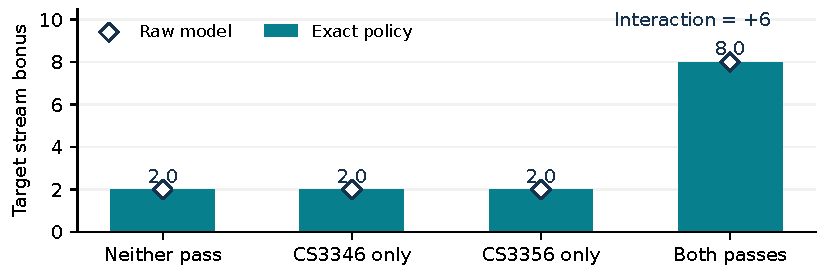
\includegraphics[width=\linewidth]{figures/stream_interaction.pdf}
\caption{Our model reproduces the stream-completion threshold in all four controlled cases. The additional six points reward finishing the chain.}
\label{fig:interaction}
\end{figure}

Grade controls reinforce this behaviour: a passed MA2509 receives its preparation benefit, while failed, in-progress and withdrawn records do not. Prerequisite-OR checks also recognise that either qualifying alternative is sufficient. These results validate our configured mechanisms; measured workload or learning benefits require a student study. A new saved-timetable intervention changes the CM finance profile with Analysis passed: MA4542 replaces MA4545, and net utility rises from 35.661 to 36.681 when only the preparation graph changes. The profile without Analysis keeps its selection. Thus a reward change can alter a close choice, while source constraints and stronger preferences can keep another timetable unchanged.

\textbf{Personalised paths across 20 student profiles.} We generated ten CM and ten CS fictional profiles with taught core completed, random GE histories and balanced desired-stream choices. With the CM waiver rule, our path checker produces 11 academic dependency paths, five advisory paths assuming the waiver and four provisional paths requiring further rule confirmation. Representative outputs appear in Table~\ref{tab:examples}. Capstones, internships and future offerings are not assumed satisfied.

\begin{table}[H]
\centering\small
\caption{Examples of the paths and obstacles our helper explains. Arrows indicate academic dependency order.}
\begin{tabular}{p{1.4in}p{2.2in}p{1.4in}}
\toprule
Student preference & Recommended route or identified obstacle & Planning result\\
\midrule
CM: Enriched Mathematics & MA3523, MA4542, MA4545 and MA4546 & Academic path\\
CS: Artificial Intelligence & CS3383 + CS4486 $\rightarrow$ CS4487 & Academic path\\
CS: Data Science & CS3402 + CS3481 $\rightarrow$ CS4480 + CS4487 & Bridge courses needed\\
CM: Financial Mathematics & {\raggedright MA3521, MA4529 + two of MA4537, EF3320 or EF4821\par} & Waiver assumed\\
\bottomrule
\end{tabular}
\label{tab:examples}
\end{table}

Before the finance-focused update, the model passed exact stream-policy validation in 10/20 of these profiles: 0/10 CM and 10/10 CS. Rejected answers used exact policy outputs. This historical result identifies the reasoning gap that motivated further training; the updated path counts above come from the revised policy checker.

The finance examples now prioritise relevant study rather than missing EF bridge passes. We retain the published prerequisite and exclusion evidence\citep{cityu-finance}, while the CM planning waiver removes prerequisite-only blocks. Actual offerings remain separate: the saved EF snapshots contain no matching CM sections. The helper therefore explains an advisory route without inventing a registerable section.

\newpage
\section{Discussion}
Our main contribution is a planner that makes the relationship between student preference and academic feasibility explicit. A desired stream shapes the reward, completed courses change the value of the next step, and the three penalties let students express their priorities. Source checks keep these preferences connected to programme requirements. EF courses without finance-study evidence also incur an extra $1.5\lambda_b$ mismatch cost; finance preparation removes that extra cost, while section permission remains binding. Earlier curriculum-only CM simulations reach 124 or 127 credits under their encoded category rules. They do not establish actual timetable feasibility. Under the current literal MA/CS-only source pool, the entering Year 1 profile has only MA1300 and MA2509 eligible and cannot form a five-course semester; its graduation audit remains incomplete. A separate CM Semester A example is correctly reported as infeasible under the five-course minimum, demonstrating that the planner can expose a constraint problem rather than hide it.

During development, we found that reliable planning depended as much on organising course evidence as on fine-tuning. Saved pages made collection reproducible when authenticated pages or security challenges restricted access. Duplicate removal, explicit major matching and source-year tracking prevented misleading combinations of otherwise plausible course information. These practical lessons shaped our emphasis on traceable recommendations.

The current evidence supports the model's usefulness for interpreting supplied information and exploring configured preferences. It does not yet establish real workload reduction or generalisation to new cohorts. The small training evaluation shares source documents, the profile studies use fictional histories, and later CM examples expose a clear reasoning gap. We therefore evaluate model answers separately from policy corrections and retain source uncertainty in the final explanation. CS experiments cover paths and semesters, rather than a verified full-degree audit.

Our next step is to combine current, cohort-consistent rules and confirmed section bundles with lecturer-reviewed workload evidence. Assessment-week deadlines and consented student study-time data would let us test the original goal of balancing workload across a semester. Independent documents, paired schedule experiments and new student cohorts should measure recommendation quality beyond policy agreement. Students should remain able to override inferred GE interests; any real-transcript study would use consent, minimal retention and clear deletion controls.

\section{Conclusion}
We built a personalised course-planning system that combines fine-tuned language understanding, source-based validation and mathematical optimisation. Students can explore streams, adjust three penalty weights and see how earlier study affects the value of later courses. Our initial test improves from 20.0\% to 93.3\%, and controlled experiments verify penalty sensitivity and dependency rewards. The updated eight-scenario timetable comparison accepts four raw Qwen answers and eight GPT answers; explicit source validation exposes unsupported sections, insufficient loads and clashes. With traceable rules and explicit feasibility checks, our helper provides a practical foundation for more informed course choices and future evidence-based workload planning.

\begin{thebibliography}{9}
\footnotesize
\setlength{\itemsep}{0pt}
\setlength{\parsep}{0pt}
\bibitem[Yang et~al.(2025)]{qwen}
A. Yang et al., ``Qwen3 Technical Report,'' arXiv:2505.09388, 2025.
\url{https://arxiv.org/abs/2505.09388}. Model: \url{https://huggingface.co/Qwen/Qwen3-8B}.

\bibitem[Dettmers et~al.(2023)]{qlora}
T. Dettmers, A. Pagnoni, A. Holtzman and L. Zettlemoyer, ``QLoRA: Efficient Finetuning of Quantized LLMs,'' 2023. \url{https://arxiv.org/abs/2305.14314}.

\bibitem[SciPy contributors()]{scipy}
SciPy contributors, ``\texttt{scipy.optimize.milp},'' official documentation.
\url{https://docs.scipy.org/doc/scipy/reference/generated/scipy.optimize.milp.html}.

\bibitem[CityUHK(2022--2026)]{cityu-programmes}
CityUHK, supplied \emph{Student Handbook 2026--27}, CM 2025-entry normative path and designated course list; CS major requirements (2026/27) and 2025-cohort normative plan; saved GE and Semester A/B timetable pages.

\bibitem[CityUHK()]{cityu-finance}
CityUHK, course catalogue and saved rule evidence for GE2260, CB3410 and EF prerequisite chains. \url{https://www.cityu.edu.hk/catalogue/ug/current/course/GE2260.htm}; \url{https://www.cityu.edu.hk/catalogue/ug/current/course/EF3320.htm}. Historical conflicts remain flagged.

\bibitem[Project experiment records(2026)]{runs}
Project experiment records, 21--24 November 2026: training, dependency rewards and the eight-profile timetable comparison; accompanying source hashes and raw outputs.
\end{thebibliography}
\end{document}
